\documentclass[a4paper,twocolumn]{article} % Document type

\ifx\pdfoutput\undefined
    %Use old Latex if PDFLatex does not work
   \usepackage[dvips]{graphicx}% To get graphics working
   \DeclareGraphicsExtensions{.eps} % Encapsulated PostScript
 \else
    %Use PDFLatex
   \usepackage[pdftex]{graphicx}% To get graphics working
   \DeclareGraphicsExtensions{.pdf,.jpg,.png,.mps} % Portable Document Format, Joint Photographic Experts Group, Portable Network Graphics, MetaPost
   \pdfcompresslevel=9
\fi

\usepackage{amsmath,amssymb}   % Contains mathematical symbols
\usepackage[ansinew]{inputenc} % Input encoding, identical to Windows 1252
\usepackage[english]{babel}    % Language
%\usepackage[round,authoryear]{natbib}  %Nice author (year) citations
\usepackage[square,numbers]{natbib}     %Nice numbered citations
%\bibliographystyle{unsrtnat}           %Unsorted bibliography
\bibliographystyle{plainnat}            %Sorted bibliography

\addtolength{\topmargin}{-30mm}% Removes 30mm from the top margin
\addtolength{\textheight}{30mm}% Adds it to the text height

\DeclareMathOperator{\tin}{\theta_\textrm{in}}
\DeclareMathOperator{\tout}{\theta_\textrm{out}}
\DeclareMathOperator{\tind}{\dot{\theta}_\textrm{in}}
\DeclareMathOperator{\toutd}{\dot{\theta}_\textrm{out}}


\begin{document}               % Begins the document

\title{Homework 2 in EL2620 Nonlinear Control}
\author{Alessio Russo \\ 911103-T192 \\ alessior@kth.se \and Enrique Cobo Jim\'enez\\
  921005-1299 \\ ejcj@kth.se}
%\date{2010-10-10}             % If you want to set the date yourself.

\maketitle                     % Generates the title




%%%%%%%%%%%%%%%%%%%%%%%%%%%%%%%%%%%%%%%%%%%%%%%%%%%%%%%%%%%%%%%%%%%%%%%%%%%%%%%%%%%
% solutions
%%%%%%%%%%%%%%%%%%%%%%%%%%%%%%%%%%%%%%%%%%%%%%%%%%%%%%%%%%%%%%%%%%%%%%%%%%%%%%%%%%%

\section*{Problem}
\label{sec:prob}
The problem considered is the analysis  of a type of 2-species population model, which is the following one:
\begin{subequations}\label{eqn:syseqs}
\begin{align}
    \frac{d x}{dt} & = x(a+bx+cy) \label{eqn:syseq1} \\
    \frac{d y}{dt} & = y(d+ex+fy) \label{eqn:syseq2}
\end{align}
\end{subequations}
Where $a,b,c,d,e,f \in \mathbb{R}$ and $x=x(t), y=y(t)$ are functions such that:
$$x(t),y(t): \mathbb{R}_0^+ \to \mathbb{R}_0^+$$
They are non negative functions starting at time $t=0$.\\
$x,y$ describe the evolution of two species on a grassy island, and depending on the value of the constants $x$ may prey on $y$, or have other kind of behaviours.\\ \\
The analysis of such model is broken down into the following five sub-problems:
\begin{enumerate}
\item {Depending on the signs of the coefficients describe the different types of populations models and label those models as: 
\begin{itemize}
\item Predator-Prey($x$ predator, $y$ prey)
\item Prey-Predator($x$ prey, $y$ predator)
\item Competitive($x$ and $y$ inhibits each other)
\item Symbiotic($x$ and $y$ benefit each other)
\end{itemize}}
\item{Consider the case when $(a,b,f,d)=(3,-1,-1,2)$. Draw the phase portrait, interpret the model and determine the type of each equilibrium for the following cases:
\begin{itemize}
\item $(c,e) = (-2,-1)$
\item $(c,e) = (-2,1)$
\item $(c,e) = (2,-1)$
\item $(c,e) = (2,1)$
\end{itemize}}
\item {Again, consider the previous questions, but analyse the model for the case $(a,e,b,f,c,d)=(1,1,0,0,-1,-1)$.}
\item {Show that the $x$- and $y$-axes are invariant for all values of the parameters $(a,b,c,d,e,f)$. Why is this a necessary feature of a population model? Assuming $(a,e,b,f,c,d)=(1,1,0,0,-1,-1)$ show that a periodic orbit exists.}
\item {Generalize the population model to $N>2$ species.}
\end{enumerate}

\section*{Solution - Question 1}
\label{sec:sol1}
The eigenvalues of the systems are given by solving the characteristic polynomial:
$$\det(\lambda I -A)=0$$
The solution, calculated using Matlab, is the following:\\
$\lambda_i=(-3.65,1.066,0.0027,-20,-20,-125,-125)^T$. Two of the poles, $\lambda_2=1.0662, \lambda_3 = 0.0027$ have positive real part thus the model is unstable.
This is because the flight dynamics is unstable and we can make the following reasoning: we expect the internal elevator state and the internal spoiler state to have very fast dynamics, since they correspond to the dynamics of the rudder servos, same for the elevator and spoiler angle. In fact  $\lambda_4,\lambda_5,\lambda_6,\lambda_7$  have large value, in an absolute sense, and those eigenvalues should corresponds to the rudder dynamics, therefore $\lambda_1,\lambda_2,\lambda_3$ should correspond to the flight dynamics. Moreover it is normal to assume that the rudder dynamics do not depend on the flight dynamics. To prove all of that, observe the matrix $A$:\begin{multline}
A=
\left[
\begin{matrix}
   -1.3936 &   0.9744  & -0.0019&   -0.5349   \\
  5.6870 &  -1.1827 &   0.0002  &-25.9398 \\
   0 &   1.0000  &       0   &      0  \\
   0  &       0    &     0  & -20.0000  \\
  0   &      0    &     0   &      0 \\
  0  &       0     &    0    &     0   \\
   0   &      0      &   0     &    0
\end{matrix}
\right.
\\
\left.
\begin{matrix}
 -0.0071  & -1.0562  &  0.4891 \\
  7.9642 & -23.8594 &  -6.2531 \\
   0        & 0  &       0\\
    0& -312.5000    &     0\\
  -20.0000        & 0 &-312.5000 \\
  0& -125.0000   &      0 \\
  0&         0 &-125.0000
\end{matrix}
\right]
\end{multline}
and notice that $\delta_e,\delta_s, x_e, x_s$ (last four rows) have dynamics that do no depend on $\alpha, \theta, \dot{\theta} $ (first three row/states), which indicates the rudder does not depend on the pitch or angle of attack, as expected. \\Then:
$$\textrm{eig}(A) = \textrm{eig}(A_1)\cup \textrm{eig}(A_2)$$
where $\textrm{eig}(A)$ denotes the eigenvalues of the matrix $A$ and $A_1 =A(\text{1:3,1:3}), A_2=(\text{4:7,4:7})$. $A_1$ represents the first 3 states, the flight dynamics, and $A_2$ represents the states of the rudder dynamics. A simple check gives that $\textrm{eig}(A_1)= (-3.6452,1.0662,0.0027)$, so the flight dynamics are unstable. \\ This can also be proven by checking the eigenvectors associated to each eigenvalue, and see that each eigenvalue is mainly associated with one state.
\section*{Solution - Question 2}
%\label{sec:sol2}
Now consider the following system:

$$
    \left\{\begin{aligned} 
      \dot{x}(t) = x(3-x+cy) \\
      \dot{y}(t) = y(2+ex-y)
    \end{aligned}\right.
$$
The equilibrium points are given by setting $\dot{x}=0, \dot{y}=0$:
$$
    \left\{\begin{aligned} 
      0 = x(3-x+cy) \\
      0 = y(2+ex-y)
    \end{aligned}\right.
$$

% From which we obtain the solutions:
% $$
%     \left\{\begin{aligned} 
%       x &= 0 \\
%       y &= 0
%     \end{aligned}\right. \cup 
%     \left\{\begin{aligned}
%      x &= 0 \\
%      y&=2+ex
%     \end{aligned}\right. \cup
%     \left\{\begin{aligned}
%      y &= 0 \\
%      x&=3+cy
%     \end{aligned}\right. \cup
%     \left\{\begin{aligned}
%      x &= 3+cy \\
%      y&= 2+ex
%     \end{aligned}\right.
% $$
Let $\mathbf{p}_i = (x_i,y_i)$ be the i-eth equilibria. The first three equilibria are given by $\mathbf{p}_1 = (0,0), \mathbf{p}_2 = (0,2), \mathbf{p}_3 = (3,0)$. The 4-th equilibria is given by:
$$
    \left\{\begin{aligned}
     x &= 3+cy \\
     y&= 2+3e+cey
    \end{aligned}\right. \Rightarrow
    \left\{\begin{aligned}
     x &= 3+c\frac{2+3e}{1-ce} \\
     y&= \frac{2+3e}{1-ce}\quad ce \neq 1
    \end{aligned}\right.
$$
Thus $\mathbf{p}_4 = ( \frac{3+2c}{1-ce}, \frac{2+3e}{1-ce})$ with $ce \neq 1$.

To study the equilibrium points we can linearise the system around those equilibrium points to study the behaviour of the system, by using the Hartman-Grobman theorem~\cite[p. 288]{Sastry:1999:Nonlinear-systems:-analysis-stability-and-control:xr}. We will therefore linearise the system around the equilibrium points, calculate the eigenvalues, and determine the equilibria based on the eigenvalues. The linearisation is given by  $\dot{\tilde{\textbf{x}_i}} = A \tilde{\textbf{x}_i}$, with $\tilde{\textbf{x}_i} = \textbf{x} - \textbf{x}_i$ and the Jacobian matrix $A = \left. \frac{\partial\textbf{f}}{\partial \textbf{x}}(\textbf{x}) \right|_{\textbf{x}=\textbf{x}_i}$. \\The Jacobian matrix in this case is:
$$
 A=
    \left[\begin{array}{cc}
    3-2x+cy  & cx\\
    ey & 2+ex-2y
    \end{array}\right]
    $$
    
Now we analyze each equilibrium point separately in order to classify them. Since we have a second-order system, we know that we can classify by looking at the eigenvalues of the Jacobian: ~\cite[p. 37]{Khalil:2002:Nonlinear-systems:vh}

\begin{itemize}
\item If they are \textbf{real}, equilibrium is going to be a stable node if both are negative, an unstable node if both are positive, and a saddle point if one is positive and the other is negative.

\item If they are \textbf{complex}, we have to look at the real part. If it is positive, we have an unstable focus; negative belongs to a stable focus, and zero implies a non-hyperbolic equilibrium.
\end{itemize}

We start from $\mathbf{p}_1 = (0,0)$. The Jacobian at this point becomes:    
$$
 A_{(0,0)}=
    \left[\begin{array}{cc}
    3  & 0\\
    0 & 2
    \end{array}\right]
$$

Whose eigenvalues are $\lambda_1 = 3$ and $\lambda_2 = 2$. Since both of them are positive, the equilibrium point $\mathbf{p}_1$ is an unstable node.

For the point $\mathbf{p}_2 = (0,2)$ the Jacobian turns out to be:
$$
 A_{(0,2)}=
    \left[\begin{array}{cc}
    3 +2c  & 0\\
    2e & -2
    \end{array}\right]
$$

And the eigenvalues becomes $\lambda_1 = 3 + 2c$ and $\lambda_2 = -2$. In this case, we have to look at the value of $c$ to classify this point. If $c<-\frac{3}{2}$ this equilibrium is a stable node; and it is a saddle point if $c > -\frac{3}{2}$.

If we have a look to the third point, $\mathbf{p}_3 = (3,0)$, whose Jacobian is:
$$
 A_{(3,0)}=
    \left[\begin{array}{cc}
    -3  & 3c\\
    0 & 3e+2
    \end{array}\right]
$$
And the eigenvalues are $\lambda_1 = -3$ and $\lambda_2 = 2+3e$. As in the previous case, the character of this point would depend of the value of $e$. If $e<-\frac{2}{3}$ this point would be a stable node; and a saddle point otherwise. 

Finally, the fourth point $\mathbf{p}_4 = \left( \frac{3+2c}{1-ce}, \frac{2+3e}{1-ce} \right)$ is strongly related to the values of $c$ and $e$, so we match each tuple $(c,e)$ with its character.

\begin{itemize}
\item For $(c,e) = (-2, -1)$, $\mathbf{p}_4 = (1,1)$, and the eigenvalues are $\lambda_1 = -2.41$ and $\lambda_2 = 0.4142$, being a saddle point.
\item For $(c,e) = (-2, 1)$, $\mathbf{p}_4 = (-\frac{1}{3},\frac{5}{3})$, and the eigenvalues are $\lambda_1 = 0.786$ and $\lambda_2 = -2.11$, being a saddle point.
\item For $(c,e) = (2, -1)$, $\mathbf{p}_4 = (\frac{7}{3},-\frac{1}{3})$, and the eigenvalues are $\lambda_1 = 0.82$ and $\lambda_2 = -2.82$, being a saddle point.
\item For $(c,e) = (2, 1)$, $\mathbf{p}_4 = (-7,-5)$, and the eigenvalues are $\lambda_1 = -2.41$ and $\lambda_2 = 14.42$, being a saddle point.
\end{itemize}

Having characterized all equilibria, we comment the phase plane for all values of $(c,e)$ given in the formulation.

\begin{enumerate}
\item $(c,e) = (-2, -1)$. The phase portrait of the system described is shown in Figure~\ref{fig:ppcomp}. As we show in the first section, this case corresponds to a \textbf{competitive} scenario, in which both species can survive either eating grass or the other. So, there are two stable nodes, $(0,2)$ if $y$ eats $x$; and $(3,0)$ otherwise.
\item $(c,e) = (-2, 1)$. The phase portrait of the system described is shown in Figure~\ref{fig:ppy}. This case belongs to \textbf{$\boldsymbol x$ prey, $\boldsymbol y$ predator}. Consequently, the unique stable node is located in $(0,2)$, since $y$ has eaten all $x$.
\item $(c,e) = (2, -1)$. The phase portrait of the system described is shown in Figure~\ref{fig:ppx}. Now we are in the dual case, in which \textbf{$\boldsymbol y$ is prey and $\boldsymbol x$ is predator}, and the stable solution corresponds to $(3,0)$.
\item $(c,e) = (2, 1)$. The phase portrait of the system described is shown in Figure~\ref{fig:ppsymb}. In this case, the society is \textbf{symbiotic}, and there is no stable point. The species will grow given the high amount of food available.
\end{enumerate}

\section*{Solution - Question 3}
\label{sec:sol3}
Now we analyse the system when the pilot is in an "emergency situation", and he is replaced by a "relay pilot" that models the fact that the pilot is panicking and he is trying to compensate the error $\theta_{\text{ref}}-\theta$ with maximum command signals. This behaviour may induce sustained oscillations in the system (PIO - Pilot Induced Oscillations). This is usual for system with slow unstable dynamics, such as the aircraft, that cannot respond fast enough to the command input. 

To analyse the PIO mode we can make use of the describing function method ~\cite[p. 280]{Khalil:2002:Nonlinear-systems:vh} to check for a possible periodic solution. Suppose the error $e(t)=\theta_{\text{ref}}-\theta$ is the input to the non linearity and also $e(t)$ is oscillating with amplitude $A$ and period $\omega$. Let $u(t)$ be the output of the non linearity  and suppose the plant is low-pass filter such that $|G(jn\omega)| \ll |G(j\omega)|$ for $n \geq 2$, then we may use the describing function method to  model the non linearity, so that it is replaced by a function $$N(A,\omega)= \frac{b_1(\omega)+ja_1(\omega)}{A}$$ where $b_1,a_1$ are the first Fourier coefficients of the signal $u(t)$. \\
This gives as output of the plant an oscillating signal of maximum amplitude: $$\textrm{max}|y(t)| \approx |G(j\omega)|\sqrt{a_1^2+b_1^2}= |G(j\omega)||N(A,\omega)|A$$ 
The describing function for a relay is:
$$N(A) = \frac{4D}{\pi A}$$
where $A$ is the amplitude of the oscillation and $D$ is the output value, in absolute sense, of the relay system, and in our case $D=0.2$.\\
To check for existence of period solution the idea is that we have sustained oscillations with pulsation $\omega$ if the open loop-gain is $1$ and the  phase-lag is $-\pi$ for that pulsation:
\begin{equation}\label{eq:cond1}
G(j\omega)N(A)=-1 \Leftrightarrow G(j\omega) = -\frac{1}{N(A)}
\end{equation}
Notice that because of that condition, the output in module has maximum amplitude:
$$\textrm{max} |y(t)| \approx  |G(j\omega)||N(A,\omega)|A = A$$ 
In our case the describing function gives no phase contribution, so we first check for which $\omega $:
\begin{equation} \label{eq:cond2}
\textrm{arg}G(j\omega)=-\pi
\end{equation}
To do so we linearised the system and analysed the Bode and Nyquist plots (figures \ref{fig:sim2bode}, \ref{fig:sim2nyquist}).\\
By checking the plots, the condition (\ref{eq:cond2}) is satisfied for $\omega \approx 2.77 \frac{\textrm{rad}}{\textrm{sec}}$: the Nyquist curve for that pulsation has imaginary part which is almost 0 and  real part $-0.402$. In fact $|G(j2.77)| = -7.92 dB \approx 0.402$.\\
Then we need to find for which $A$ we may obtain oscillations, by using the condition (\ref{eq:cond1}):
$$ G(j2.77) \approx -0.402 = -\frac{\pi A}{4D} \Rightarrow A \approx 0.1024$$
The period of the oscillation is given by: $$\frac{2\pi}{\omega} = \frac{2\pi}{2.77}\approx 2.27 \textrm{ seconds} $$ By simulating the system we see the aircraft oscillating around the set point $1 \text{rad}$ of $\pm 0.1 \text{rad}$ with period $\sim 2.34$ seconds, which is almost what we obtained with the describing function analysis. So the prediction, using the describing function analysis, gives very good results for this case.
\section*{Solution - Question 4}
%\label{sec:sol4}

In this question we analyze two different designs. Both of them change $L$ and $K_f$ to a faster design, and the difference between them are the filter time constant $T_f$, from 0.3 to 0.03 seconds. 

The process we are going to follow is the one described in question \textbf{3}. 

\begin{enumerate}
\item We start analyzing \textit{design2}. Bode and Nyquist plot are shown in figures \ref{fig:bode2} and \ref{fig:nyquist2} respectively. 

From this analysis, we get that the condition (\ref{eq:cond2}) is satisfied for  $\omega \approx 4.41 \frac{\textrm{rad}}{\textrm{sec}}$. In addition, the Nyquist curve in this point gives real part -0.4212 and imaginary part almost 0. If we apply (\ref{eq:cond1}) we obtain the amplitude:
$$ G(j4.41) \approx -0.4212 = -\frac{\pi A}{4D} \Rightarrow A \approx 0.1073$$

And the period turns out to be 1.428 seconds. 

\item Now we focus in \textit{design3}. Both Bode and Nyquist curves can be found in figures \ref{fig:bode3} and \ref{fig:nyquist3}. 

Following the same proceeding, the condition (\ref{eq:cond2}) is satisfied for this design for $\omega \approx 8.15 \frac{\textrm{rad}}{\textrm{sec}}$. The Nyquist curve for this point shows, for this $\omega$, a real part of -0.25, and an almost 0 imaginary part. Now, applying condition (\ref{eq:cond1}):
$$ G(j8.15) \approx -0.25 = -\frac{\pi A}{4D} \Rightarrow A \approx 0.0637$$
And the period in this case is 0.771 seconds. 
\end{enumerate}

Now we compare all designs under analysis. This comparative is depicted in figure \ref{fig:comparative}. Some conclusions can be obtained from this plots: 

\begin{enumerate}
\item The concordance between the theoretical and  simulated values are very good, being the amplitude 0.106 and 0.071, and the period 1.479 and 0.853 seconds; for \textit{design2} and \textit{design3}, respectively.

\item If we compare the values from \textit{design2} with those obtained under \textit{design1}, we can see that the amplitude is about the same in \textit{design2}, whereas the period is smaller. This could be explained by considering the fact that the system now is faster but the pilot command is still slow:  so the oscillations have the same amplitude but now happens more frequently.

\item Regarding \textit{design3}, we can see that both amplitude and period has decreased compared to those obtained under \textit{design1}. Now the faster reaction of the pilot are captured by the low pass filter: this reduces the amplitude of the oscillations, because the pilot command is faster, despite making them more frequent (because of the fact that the system is faster).
\end{enumerate}


\section*{Solution - Question 5}
%\label{sec:sol5}
In this question we suggest a new design in order to improve the performance of the system. This new design is based on a combination between \textit{design1} and the filter time constant set in \textit{design3}. 

Under these conditions we analyze the system, as explained in question \textbf{3}. The reference plots for the Bode and Nyquist curves are depicted in figures \ref{fig:bodeimp} and \ref{fig:nyquistimp}. 

Now we apply condition (\ref{eq:cond2}). In this case, we obtain $\omega \approx 5.99 \frac{\textrm{rad}}{\textrm{sec}}$ (period of 1.0489 seconds). The Nyquist point for this pulsation gives a real part of -0.147, and a imaginary part almost 0. So, condition (\ref{eq:cond1}) gives us the amplitude of: 

$$ G(j5.99) \approx -0.147 = -\frac{\pi A}{4D} \Rightarrow A \approx 0.0374$$

Figure \ref{fig:improved} shows this suggested design in contrast with the other designs analyzed along this work. We first check the accuracy of the results obtained. The simulated amplitude is 0.043 radians, and the period is 1.128 seconds.

Comparing all design, we can see that our improved system gives the smallest amplitude of the oscillations. Now, this system is slower and also the pilot signal is faster, which is the key point to understand why now this amplitude is small. 

If we look at the period, we can see that it is smaller than the one in \textit{design3}, but greater that the obtained under \textit{design1}.  \\
Overall it's a plausible model since the period is still high, so the pilot has not to do many quick movements. \\ \\
Another way to reduce the PIO amplitude would be to change the filter on the pilot command in order to change the Nyquist locus.



%%%%%%%%%%%%%%%%%%%%%%%%%%%%%%%%%%%%%%%%%%%%%%%%%%%%%%%%%%%%%%%%%%%%%%%%%%%%%%%%%%%
% Example 1
%%%%%%%%%%%%%%%%%%%%%%%%%%%%%%%%%%%%%%%%%%%%%%%%%%%%%%%%%%%%%%%%%%%%%%%%%%%%%%%%%%%

% \section*{Problem 1 -- Behavior of a nonlinear system}
% \label{sec:prob1}
% Study the behavior of the system
% \begin{subequations}\label{eqn:PPSystem}
% \begin{align}
%     \frac{d x}{dt} & = y \label{eqn:PPSystem1} \\
%     \frac{d y}{dt} & = -2x -2y -4 x^2 \label{eqn:PPSystem2}
% \end{align}
% \end{subequations}
% with regard to its initial value and assess if the system is globally asymptotically stable.

% We have chosen a solution strategy based on the phase portrait and broken down the problem into the following three subproblems:
% \begin{enumerate}
%   \item Draw the phase portrait of the system.
%   \item How many equilibrium points does the system have, where are they located, and what type of equilibrium points are they?
%   \item Is the system globally asymptotically stable?  That is, do all trajectories lead to the same equilibrium point?
% \end{enumerate}

% \section*{Solution 1 -- Behavior of a nonlinear system}
% \label{sec:sol1}

% \begin{enumerate}
%   \item The phase portrait of the system described by \eqref{eqn:PPSystem} is shown in Figure~\ref{fig:pplane}.

%   \item The system has two equilibrium points, \mbox{(0,0)} and \mbox{($-\frac{1}{2}$,0)}.  They were computed by setting the right hand side of \eqref{eqn:PPSystem} equal to zero
% \begin{align*}
%     \begin{array}{rl}
%     y & =0  \\
%     -2x -2y -4 x^2 & = 0
%     \end{array} \; \Rightarrow
%     \begin{array}{rl}
%       y & =0 \\
%       x (1+2x) & =0
%     \end{array}.
% \end{align*}
% Both points are marked by large dots in Figure~\ref{fig:pplane}.

% Let us now characterize the equilibrium points. The Hartman-Grobman theorem~\cite[p. 288]{Sastry:1999:Nonlinear-systems:-analysis-stability-and-control:xr} states that the behavior of a nonlinear system near a hyperbolic equilibrium is qualitatively the same as its linearization at the equilibrium point. An equilibrium is by definition hyperbolic if the real part of the eigenvalues of the Jacobian matrix are all non-zero. We will therefore linearize the system \eqref{eqn:PPSystem} around both equilibrium points, calculate the eigenvalues, check if the points are hyperbolic, and determine the type of the equilibria based on the eigenvalues.

% The linearization of an autonomous nonlinear system $\dot{\textbf{x}} = \textbf{f}(\textbf{x})$ around an equilibrium point, given by $\textbf{f}(\textbf{x}_0) = 0$, is $\dot{\tilde{\textbf{x}}} = A \tilde{\textbf{x}}$, with $\tilde{\textbf{x}} = \textbf{x} - \textbf{x}_0$ and the Jacobian matrix $A = \left. \frac{\partial\textbf{f}}{\partial \textbf{x}}(\textbf{x}) \right|_{\textbf{x}=\textbf{x}_0}$. The Jacobian matrix is calculated to be
% \begin{equation*}
%     \frac{\partial\textbf{f}}{\partial \textbf{x}}(\textbf{x}) =
%     \left[\begin{array}{cc}
%     0 & 1 \\
%     -2 -8x & -2
%     \end{array}\right],
% \end{equation*}
% which for the two equilibrium points turns out to be
% \begin{equation*}
%     A_{(0,0)} =
%     \left[\begin{array}{cc}
%     0 & 1 \\
%     -2 & -2
%     \end{array}\right], \; A_{(-\frac{1}{2},0)} =
%     \left[\begin{array}{cc}
%     0 & 1 \\
%     2 & -2
%     \end{array}\right].
% \end{equation*}
% The eigenvalues of the Jacobian matrix are given by the characteristic equation
% \begin{equation*}
%     \det(\lambda I - A) = 0.
% \end{equation*}
% The characteristic equation of the system linearized around \mbox{(0,0)} is
% \begin{equation*}
%     \lambda^2 +2 \lambda + 2 = 0,
% \end{equation*}
% which gives the eigenvalues $\lambda_{1,2} = -1 \pm j$. The characteristic equation of the system linearized around \mbox{($-\frac{1}{2}$,0)} is
% \begin{equation*}
%     \lambda^2 +2 \lambda - 2 = 0,
% \end{equation*}
% which gives the eigenvalues $\lambda_1 = \sqrt{3} -1 \approx 0.73$ and $\lambda_2 = -1 -\sqrt{3} \approx -2.73$. Both equilibrium points are hence hyperbolic and we can characterize them based on the eigenvalues of the Jacobian matrix of the linearized systems.  The eigenvalues tell us that we have a stable focus at \mbox{(0,0)} and a saddle point at \mbox{($-\frac{1}{2}$,0)}. This is easily verified by looking at Figure~\ref{fig:pplane}.

%   \item Only trajectories starting within the shaded region and its extension above the part of the phase portrait shown in Figure~\ref{fig:pplane} leads to the stable focus. It is therefore obvious that the system is not globally asymptotically stable.
% \end{enumerate}

% \noindent \textbf{Answer:} The system has two equilibrium points; a stable focus at \mbox{(0,0)} and a saddle point at \mbox{($-\frac{1}{2}$,0)}. It is not globally asymptotically stable.

% We have learned how to analyze the behavior of autonomous nonlinear systems with two states by drawing the phase portrait and characterizing the equilibrium points of the system.



%%%%%%%%%%%%%%%%%%%%%%%%%%%%%%%%%%%%%%%%%%%%%%%%%%%%%%%%%%%%%%%%%%%%%%%%%%%%%%%%%%%
% The bibliography
%%%%%%%%%%%%%%%%%%%%%%%%%%%%%%%%%%%%%%%%%%%%%%%%%%%%%%%%%%%%%%%%%%%%%%%%%%%%%%%%%%%
%\bibliography{Bibliography_template} %Read the bibliography from a separate file

\begin{thebibliography}{99}
\bibitem[Exercises(2015)]{Exercises:2015}
Henning Schmidt et al.
\newblock \emph{Exercises and Homework for EL2620 Nonlinear Control}.
\newblock Automatic Control Dept. at KTH. October 2015.

\bibitem[Khalil(2002)]{Khalil:2002:Nonlinear-systems:vh}
Hassan~K Khalil.
\newblock \emph{Nonlinear systems}.
\newblock Prentice Hall, Upper Saddle river, 3. edition, 2002.
\newblock ISBN 0-13-067389-7.

\bibitem[Oppenheim(2002)]{Oppenheim:2002:Signals-and-systems}
Alan~V Oppenheim.
\newblock \emph{Signals and systems}.
\newblock Prentice Hall, 2. edition, 1996.
\newblock ISBN 0-13-814757-4 .

% \bibitem[Oetiker et~al.(2008)Oetiker, Partl, Hyna, and
%   Schlegl]{Oetiker:2008:TheNotSoShortIntroductiontoLaTeXe}
% Tobias Oetiker, Hubert Partl, Irene Hyna, and Elisabeth Schlegl.
% \newblock \emph{The Not So Short Introduction to \LaTeXe}.
% \newblock Oetiker, OETIKER+PARTNER AG, Aarweg 15, 4600 Olten, Switzerland,
%   2008.
% \newblock http://www.ctan.org/info/lshort/.

% \bibitem[Sastry(1999)]{Sastry:1999:Nonlinear-systems:-analysis-stability-and-c%
% ontrol:xr}
% Shankar Sastry.
% \newblock \emph{Nonlinear systems: analysis, stability, and control},
%   volume~10.
% \newblock Springer, New York, N.Y., 1999.
% \newblock ISBN 0-387-98513-1.
\end{thebibliography}


%%%%%%%%%%%%%%%%%%%%%%%%%%%%%%%%%%%%%%%%%%%%%%%%%%%%%%%%%%%%%%%%%%%%%%%%%%%%%%%%%%%
% Place your figures and tables at the end of the document starting on a new page
%%%%%%%%%%%%%%%%%%%%%%%%%%%%%%%%%%%%%%%%%%%%%%%%%%%%%%%%%%%%%%%%%%%%%%%%%%%%%%%%%%%
\clearpage % Ends the current page and causes all figures and tables to be printed
\begin{figure*}[p] % The * makes the figure span both columns, p places the figure on a float page
  \begin{center}
 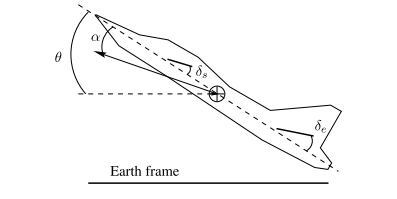
\includegraphics[width=0.7\textwidth]{images/problem/aircraft.png}
  \end{center}
  \caption{Aircraft model considered, obtained from ~\cite[p. 15]{Exercises:2015}.}
  \label{fig:aircraft}
\end{figure*}
\begin{figure*}[p] % The * makes the figure span both columns, p places the figure on a float page
  \begin{center}
 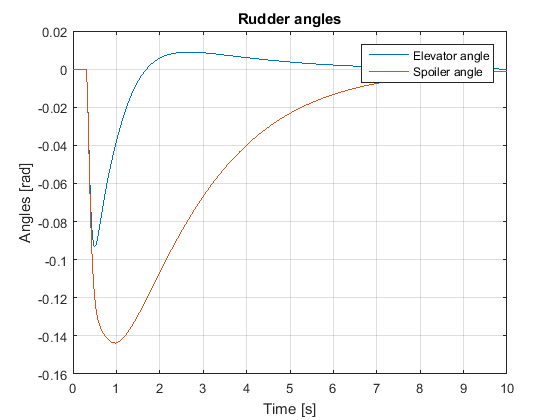
\includegraphics[width=0.8\textwidth]{images/sol2/rudderangles1.png}
  \end{center}
  \caption{Plot of the rudder angles by simulating the system using the PD-Controller as model for the pilot and \emph{design1} settings.}
  \label{fig:rangles1}
\end{figure*}

\begin{figure*}[p] % The * makes the figure span both columns, p places the figure on a float page
  \begin{center}
 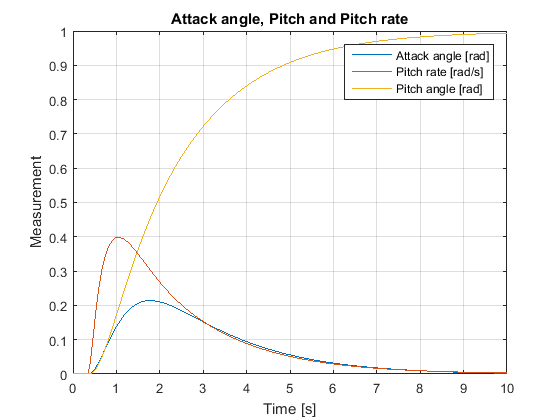
\includegraphics[width=0.8\textwidth]{images/sol2/rudderangles2.png}
  \end{center}
  \caption{Plot of the angle of attack, pitch and pitch rate by simulating the system using the PD-Controller as model for the pilot and \emph{design1} settings.}
  \label{fig:rangles2}
\end{figure*}

%solution 3
\begin{figure*}[p] % The * makes the figure span both columns, p places the figure on a float page
  \begin{center}
 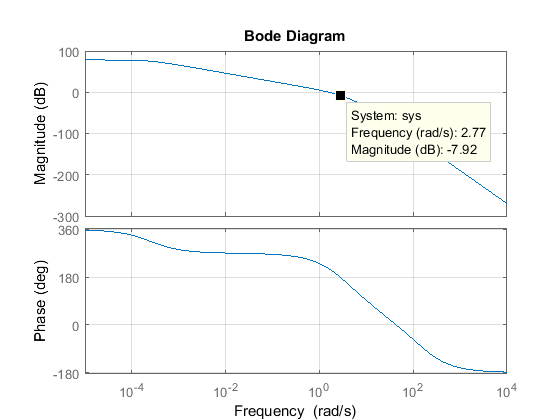
\includegraphics[width=0.8\textwidth]{images/sol3/bodeol2.png}
  \end{center}
  \caption{Bode plot of the linearised open loop using the relay model for the pilot and \emph{design1} settings.}
  \label{fig:sim2bode}
\end{figure*}

\begin{figure*}[p] % The * makes the figure span both columns, p places the figure on a float page
  \begin{center}
 \includegraphics[width=0.8\textwidth]{images/sol3/nyquist2.png}
  \end{center}
  \caption{Nyquist plot of the linearised open loop using the relay model for the pilot and \emph{design1} settings.}
  \label{fig:sim2nyquist}
\end{figure*}

% \begin{figure*}[p] % The * makes the figure span both columns, p places the figure on a float page
%   \begin{center}
%  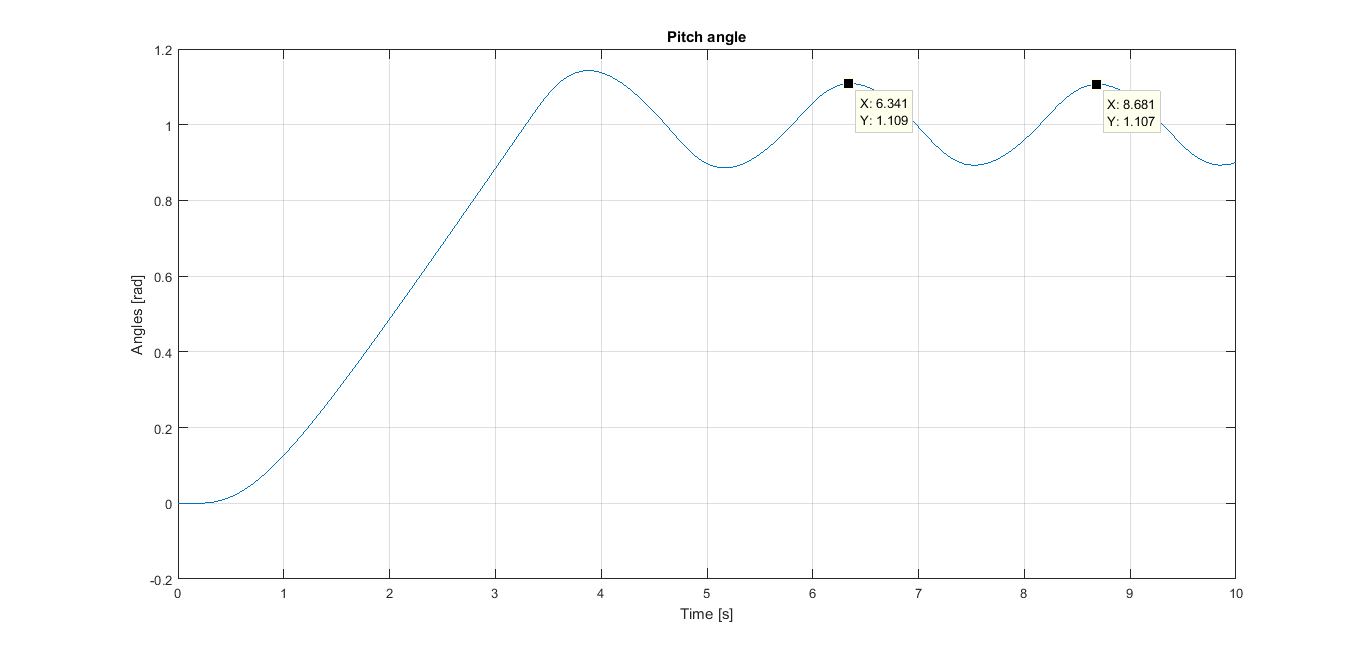
\includegraphics[width=0.8\textwidth]{images/sol3/oscillations.png}
%   \end{center}
%   \caption{Plot of the pitch angle by simulating the system using the relay  model for the pilot and \emph{design1} settings.}
%   \label{fig:sim2pitch}
% \end{figure*}

%solution 4
\begin{figure*}[p] % The * makes the figure span both columns, p places the figure on a float page
  \begin{center}
 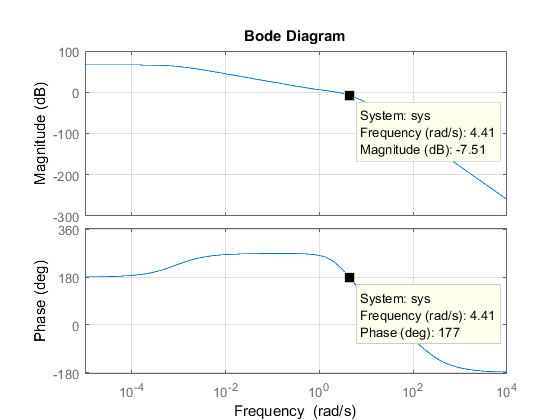
\includegraphics[width=0.8\textwidth]{images/sol4/bodeplot2.png}
  \end{center}
  \caption{Bode plot of the linearised open loop using the relay model for the pilot and \emph{design2} settings.}
  \label{fig:bode2}
\end{figure*}

\begin{figure*}[p] % The * makes the figure span both columns, p places the figure on a float page
  \begin{center}
 \includegraphics[width=0.8\textwidth]{images/sol4/nyquist2.png}
  \end{center}
  \caption{Nyquist plot of the linearised open loop using the relay model for the pilot and \emph{design2} settings.}
  \label{fig:nyquist2}
\end{figure*}
\begin{figure*}[p] % The * makes the figure span both columns, p places the figure on a float page
  \begin{center}
 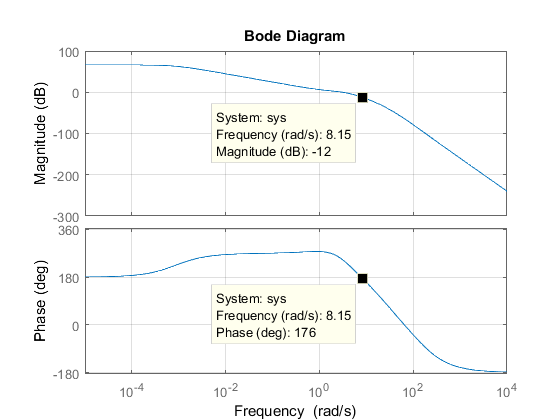
\includegraphics[width=0.8\textwidth]{images/sol4/bodeplot3.png}
  \end{center}
  \caption{Bode plot of the linearised open loop using the relay model for the pilot and \emph{design3} settings.}
  \label{fig:bode3}
\end{figure*}

\begin{figure*}[p] % The * makes the figure span both columns, p places the figure on a float page
  \begin{center}
 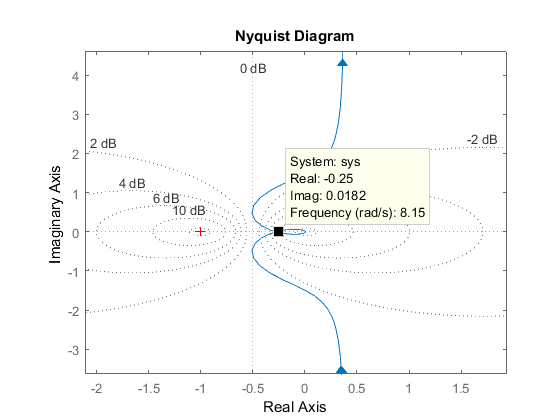
\includegraphics[width=0.8\textwidth]{images/sol4/nyquist3.png}
  \end{center}
  \caption{Nyquist plot of the linearised open loop using the relay model for the pilot and \emph{design3} settings.}
  \label{fig:nyquist3}
\end{figure*}

\begin{figure*}[p] % The * makes the figure span both columns, p places the figure on a float page
  \begin{center}
 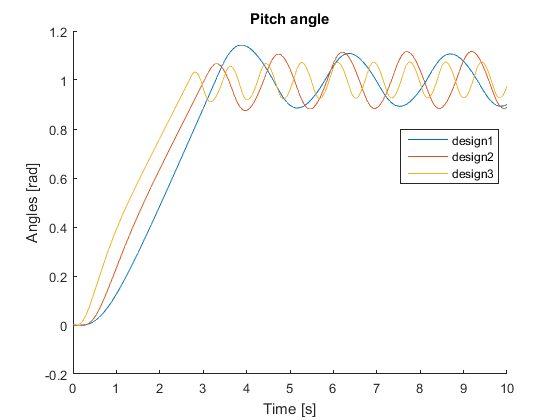
\includegraphics[width=0.8\textwidth]{images/sol4/comparative.png}
  \end{center}
  \caption{Plots of the pitch angle by simulating the system using the relay model for the pilot and \emph{design1}, \emph{design2} and \emph{design3} settings.}
  \label{fig:comparative}
\end{figure*}

%solution5
\begin{figure*}[p] % The * makes the figure span both columns, p places the figure on a float page
  \begin{center}
 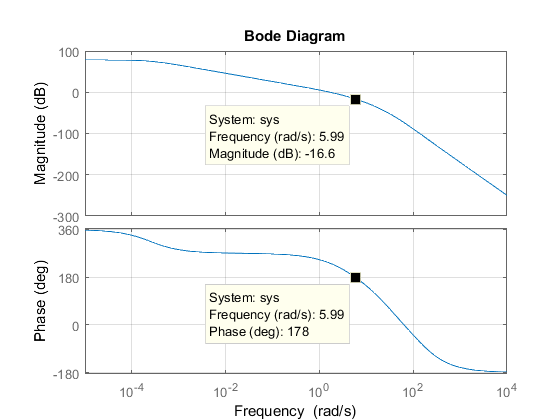
\includegraphics[width=0.8\textwidth]{images/sol5/bodeimp.png}
  \end{center}
  \caption{Bode plot of the linearised open loop using the relay model for the pilot and suggested design.}
  \label{fig:bodeimp}
\end{figure*}

\begin{figure*}[p] % The * makes the figure span both columns, p places the figure on a float page
  \begin{center}
 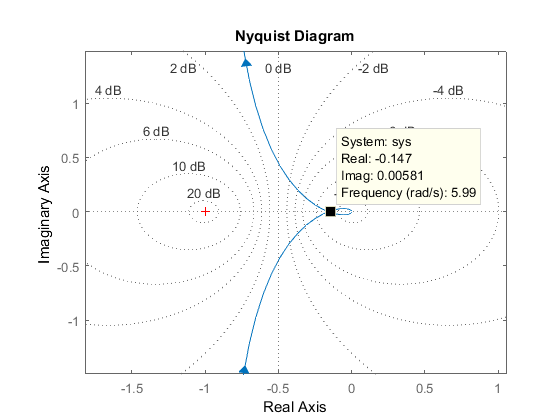
\includegraphics[width=0.8\textwidth]{images/sol5/nyquistimp.png}
  \end{center}
  \caption{Nyquist plot of the linearised open loop using the relay model for the pilot suggested design.}
  \label{fig:nyquistimp}
\end{figure*}
\begin{figure*}[p] % The * makes the figure span both columns, p places the figure on a float page
  \begin{center}
 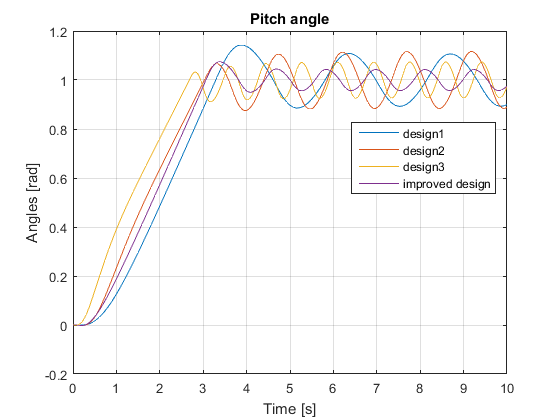
\includegraphics[width=0.8\textwidth]{images/sol5/improved.png}
  \end{center}
  \caption{Plots of the pitch angle by simulating the system using the relay model for the pilot and \emph{design1}, \emph{design2} and \emph{design3} settings, comparing them to the improved design suggested in question \textbf{5}.}
  \label{fig:improved}
\end{figure*}

%solution6

\begin{figure*}[p] % The * makes the figure span both columns, p places the figure on a float page
  \begin{center}
 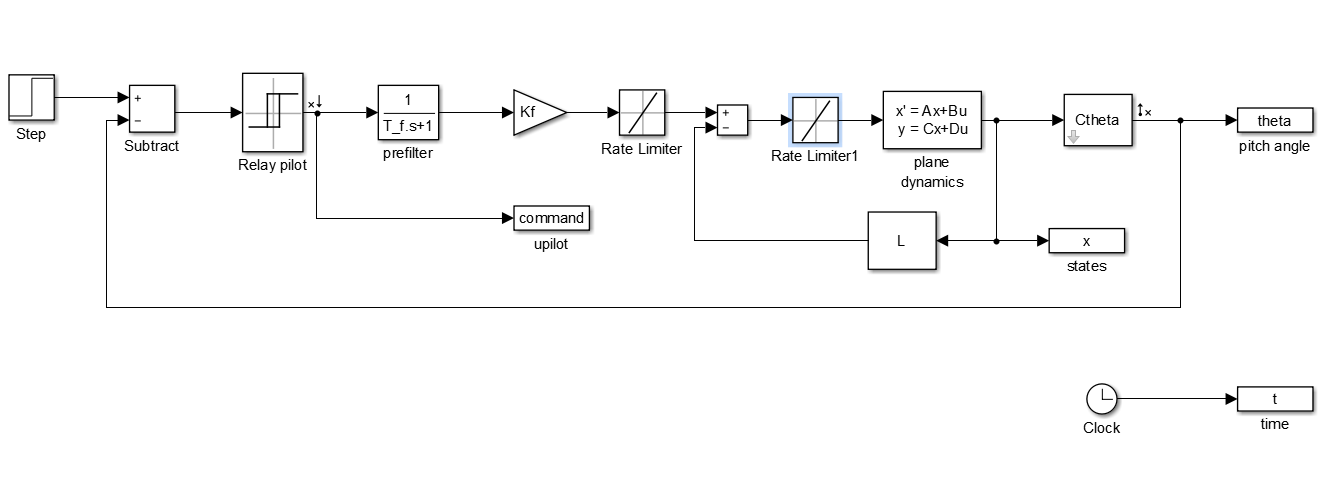
\includegraphics[width=\textwidth]{images/sol6/figcircuit.png}
  \end{center}
  \caption{Simulink model of the aircraft including the rate limiters applied on both the pilot command and on the sum of the pilot command and feedback command.}
  \label{fig:sol6circuit}
\end{figure*}


\begin{figure*}[p] % The * makes the figure span both columns, p places the figure on a float page
  \begin{center}
 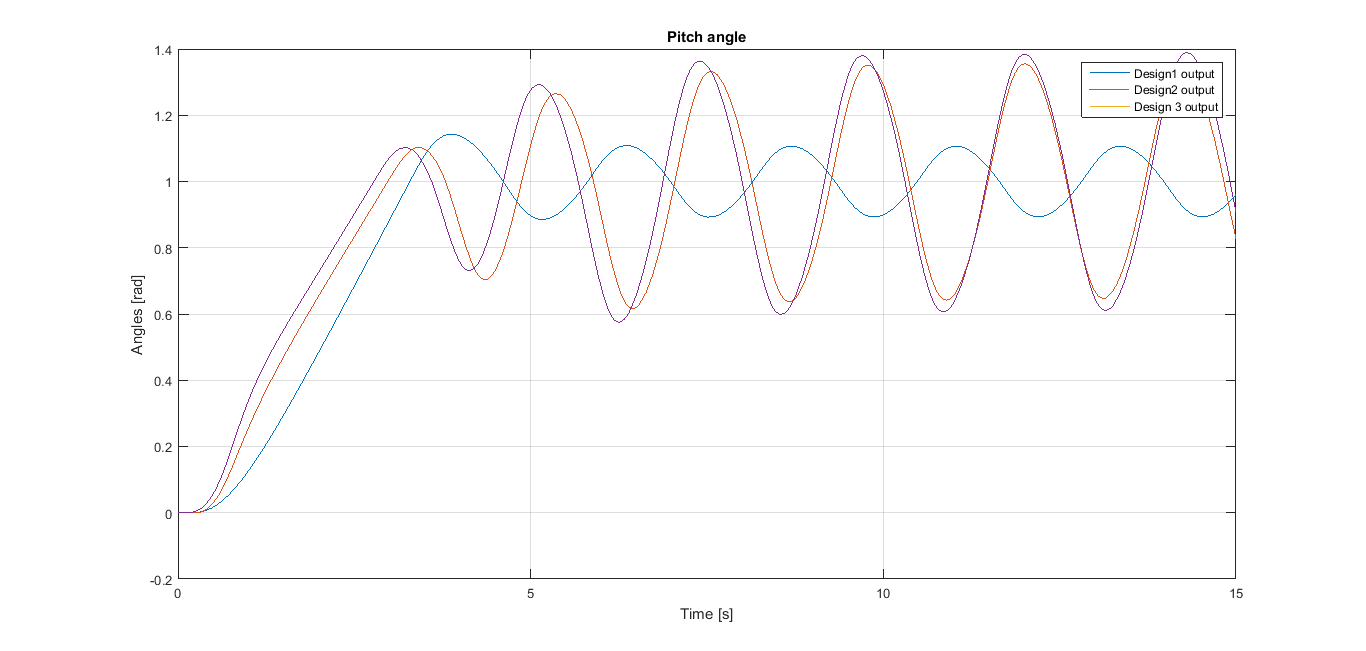
\includegraphics[width=0.8\textwidth]{images/sol6/fig1lowlimit.png}
  \end{center}
  \caption{Pitch angle plot for the various design using a rate limit $r=0.5$.}
  \label{fig:sol6lowlimit}
\end{figure*}

\begin{figure*}[p] % The * makes the figure span both columns, p places the figure on a float page
  \begin{center}
 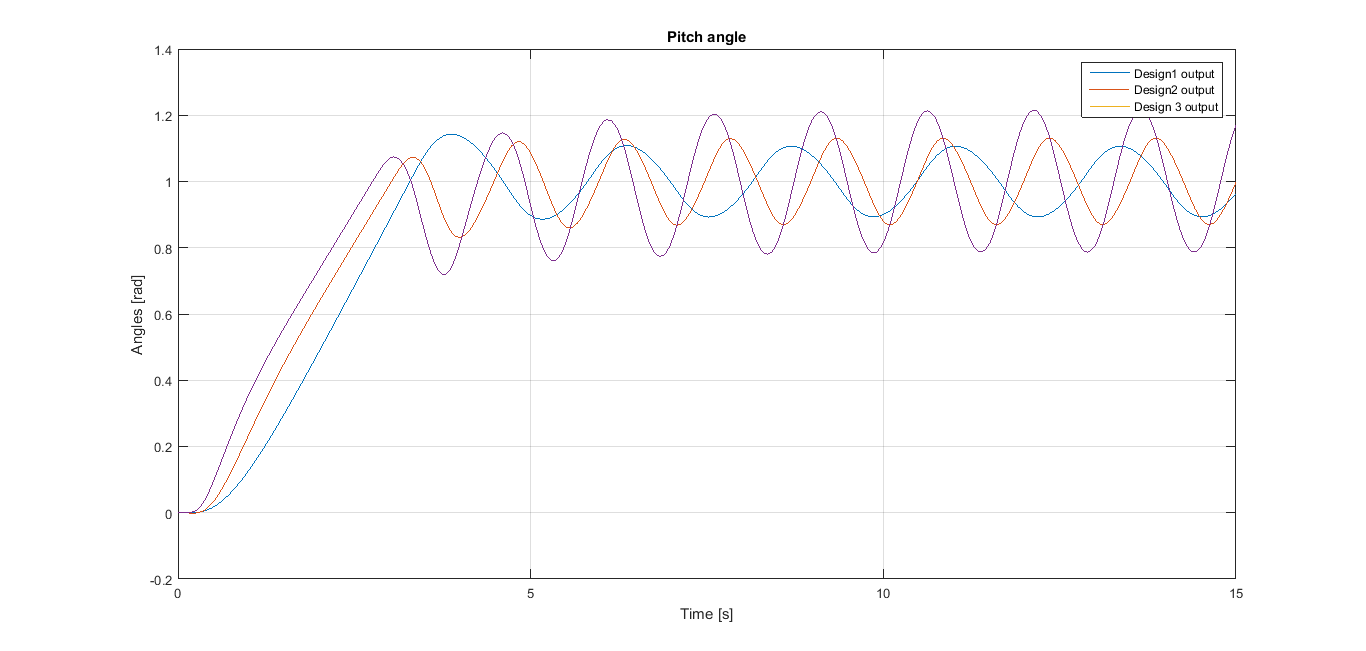
\includegraphics[width=0.8\textwidth]{images/sol6/fig2highlimit.png}
  \end{center}
  \caption{Pitch angle plot for the various design using a rate limit $r=1$.}
  \label{fig:sol6highlimit}
\end{figure*}


\begin{figure*}[p] % The * makes the figure span both columns, p places the figure on a float page
  \begin{center}
 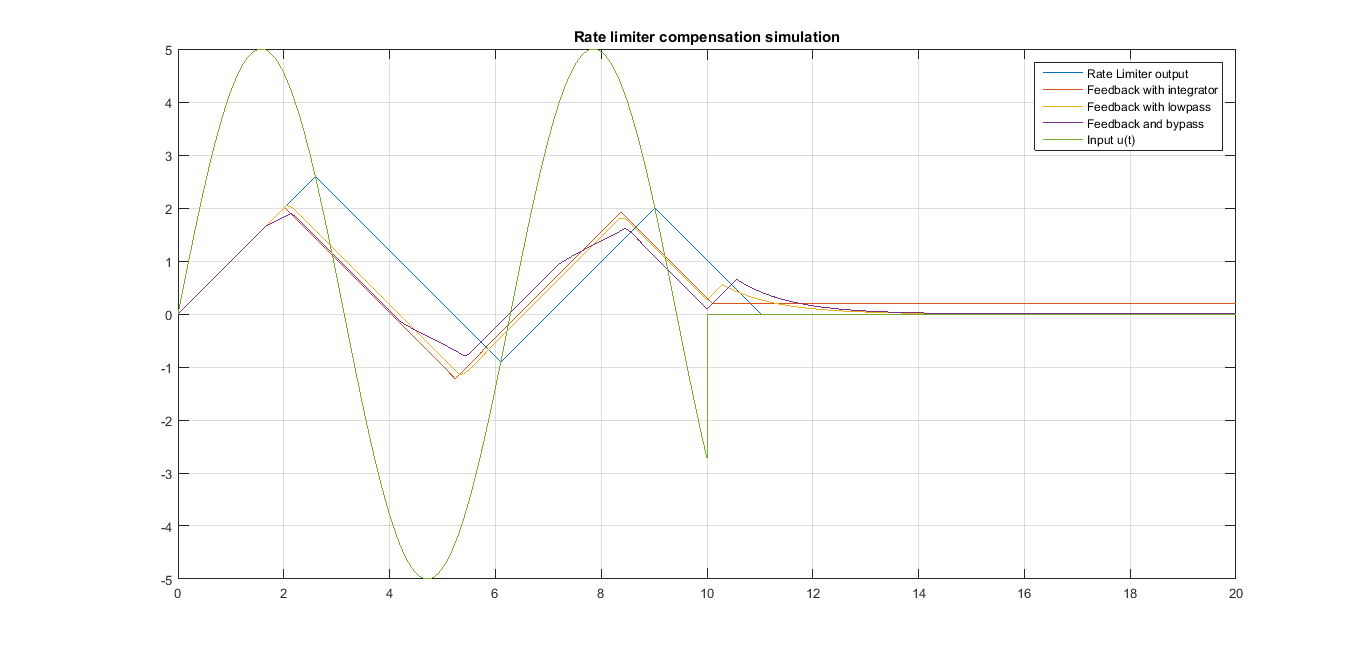
\includegraphics[width=0.8\textwidth]{images/sol6/simulationfilters.png}
  \end{center}
  \caption{Simulation of the various rate limiter filters for an input signal $u(t)=5\sin(t)$ for $t \leq 10$, $u(t)=0$ for $t > 10$. The rate limiters have rate limit value $r=1$.}
  \label{fig:simfilters}
\end{figure*}
\begin{figure*}[p] % The * makes the figure span both columns, p places the figure on a float page
  \begin{center}
 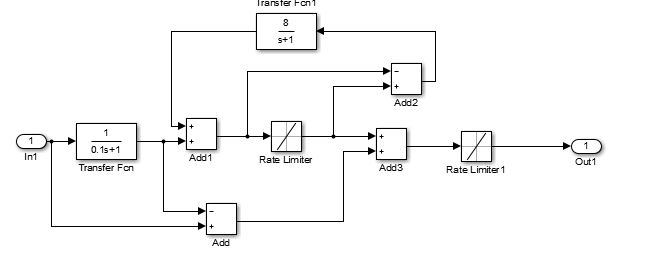
\includegraphics[width=0.8\textwidth]{images/sol6/filter.png}
  \end{center}
  \caption{Rate limiter filter with feedback and bypass [3].}
  \label{fig:filter}
\end{figure*}


\end{document}      % End of the document
